\documentclass[tikz, 10pt, convert={outfile=\jobname.svg}]{standalone}
\usepackage{times}
\usepackage{physics}
\usetikzlibrary{shapes.arrows, arrows, arrows.meta, shapes, positioning, decorations.pathmorphing, calc, patterns,decorations.markings, decorations.pathreplacing, fit, backgrounds}

\tikzset{
    myarrow/.style={
        draw,
        fill=white,
        single arrow,
        minimum height=5ex,
        line width=0.15ex,
        single arrow head extend=1ex
    },
    dummy/.style={
        minimum width=1cm,
        inner sep=0mm,
        align=center,
        minimum height=0.35cm
    },
    element/.style={
        ellipse,
        draw,
        inner sep=0mm,
        align=center,
        minimum height=1.45cm,
        minimum width=1.8cm
    },
    carre/.style = {
        rectangle,
        %        draw,
        minimum width=1.4cm,
        minimum height=1.4cm, 
        rounded corners=0.5pt, 
        inner sep=0.8mm
    },
    interaction/.style = {
        shorten >=1.5ex, 
        shorten <=1.5ex, 
        line width=2.5pt
    },
    texte/.style = {
        text height=1.5ex,
        align=center, 
        text depth=.25ex
    }
}%

%% colors
\usepackage{color}
\definecolor{bleu}{HTML}{1732a6}
\definecolor{bleu2}{HTML}{77A6EE}
\definecolor{jaune}{HTML}{ffae00}
\definecolor{rouge}{HTML}{BB0909}
\definecolor{vert}{HTML}{008000}
\definecolor{vertclair}{HTML}{98DF98}
\definecolor{orange}{HTML}{f2903f}
\definecolor{bleuclair}{HTML}{4c7ebf}


\newcommand*{\ii}{\text{i}}
\newcommand*{\e}{\text{e}}
\newcommand*{\kT}{k_\text{B}T}

% Notation abbreviations
\newcommand{\Om}{\Omega_\text{mec}}
\newcommand{\omL}{\omega_\text{las}}
\newcommand{\eff}{\text{eff}}
\newcommand{\kB}{k_\text{B}}
\newcommand{\m}{\text{m}}
\newcommand{\dXa}{\delta\hat{X}_a}
\newcommand{\dPa}{\delta\hat{P}_a}
\newcommand{\dXd}{\delta\hat{X}_d}
\newcommand{\dPd}{\delta\hat{P}_d}
\newcommand{\da}{\delta\hat{a}}
\newcommand{\db}{\delta\hat{b}}
\newcommand{\dq}{\delta\hat{q}}
\newcommand{\deltp}{\delta\hat{p}}  %% \dp already exists
\newcommand{\deltd}{\delta\hat{d}}  %% \dd already exists
\newcommand{\etaL}{\eta_\text{laser}} 
\newcommand{\etaC}{\eta_\text{conv}} 
\newcommand{\mean}[1]{\langle #1 \rangle}

\newcommand{\opt}{\text{opt}}
\newcommand{\Nm}{\bar{n}_\text{m}}
\newcommand{\Nopt}{\bar{n}_\text{opt}}
\newcommand{\Neff}{{n}_\text{eff}}


\begin{document}
    \small
        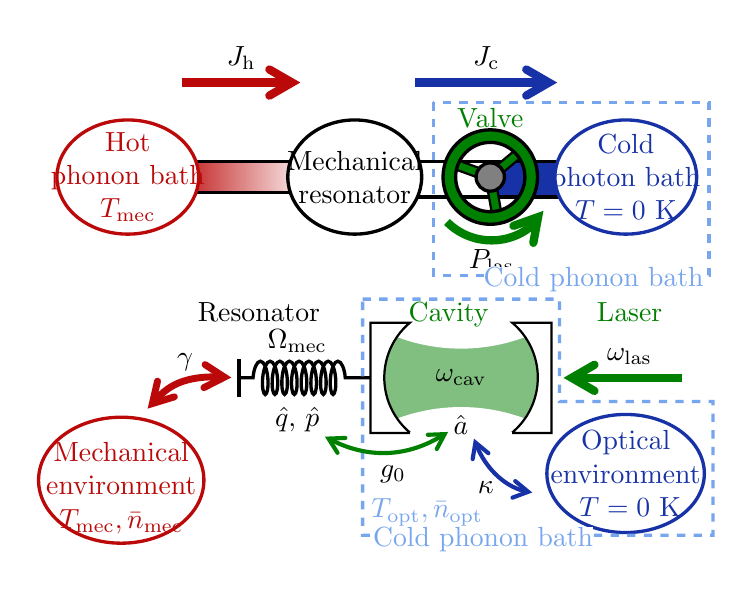
\begin{tikzpicture}[auto, >=angle 60, line width=1.2pt]
            \begin{scope}
                \node[dummy] (sys) {};
                \node[left=1.84cm of sys, dummy] (hot) {};
                \node[right=2.4cm of sys, dummy] (cold) {};
                \def\hlC{1.2}
                \shadedraw[shading=axis, left color=rouge](hot.north east) rectangle (sys.south west);
                \draw[black, fill=bleu] (cold.north west) rectangle +(-\hlC, -0.45);
                \draw[black, fill=white] (sys.north east) rectangle +(\hlC, -0.45);
                
                \node[element, minimum width=1.7cm, fill=white] at (sys) (s) {};
                \node[element, rouge, fill=white] at (hot) (h) {};
                \node[element, bleu, fill=white] at (cold) (c) {};
                \node[dummy] at (s.center) {Mechanical\\resonator};
                \node[dummy, yshift=0mm, rouge] at (h.center) {Hot\\phonon bath\\$T_\text{mec}$};
                \node[dummy, yshift=0mm, bleu] at (c.center) {Cold\\photon bath\\$T = 0$ K};
                
                \node[inner sep=0mm] at ($(sys.east) + (\hlC, 0)$) (middle) {};     
                \node[inner sep=0mm] at ($(sys.west) + (-0.92, 0)$) (middle2) {};     
                \def\w{0.06};       
                \draw[fill=vert, line width=0.8pt, rotate around={40:(middle)}] ($(middle) + (0, \w)$) rectangle +(0.45, -2*\w); 
                \draw[fill=vert, line width=0.8pt, rotate around={280:(middle)}] ($(middle) + (0, \w)$) rectangle +(0.45, -2*\w); 
                \draw[fill=vert, line width=0.8pt, rotate around={160:(middle)}] ($(middle) + (0, \w)$) rectangle +(0.45, -2*\w); 
                \draw[fill=gray] (middle) circle (0.18);
                
                \node[vert] at ($(middle) + (0, 0.75)$) {Valve};
                
                \draw[even odd rule, fill=vert] (middle) circle (0.6) (middle) circle (0.44);
                \draw[vert, line width=3pt] ($(middle) + (-0.55, -0.57)$) arc (225:315:0.8) node[midway, black, below, align=center, yshift=0.5mm] {$P_\text{las}$\\[-0.45cm]};
                \draw[decorate, decoration={ markings, mark=at position 0.91 with
                    {\arrow[vert, line width=3pt, rotate=-8]{>}};}] (middle) circle (0.8);
                
                %% effective cold bath
                \draw[dashed, bleu2] (1,0.95) rectangle (4.5,-1.25);
                \node[bleu2, fill=white, inner sep=0mm, anchor=east, yshift=-0.5mm] at (4.45, -1.25) {Cold phonon bath};
                
                
                \draw[<-, rouge, line width=3pt] ($(middle2) + (0.75, 1.2)$) -- +(-1.5, 0) node[midway, above, black] (Jh) {$J_\text{h}$};            
                \draw[->, bleu, line width=3pt] ($(middle) + (-0.95, 1.2)$) -- +(1.8, 0) node[midway, above, black] {$J_\text{c}$};            
        \end{scope}
        \begin{scope}[shift={(0.2 cm,-2.55 cm)}]
            %%% cavity
            \def\ch{0.7};
            \def\cw{0.5};
            \def\cl{1.8};
            \draw[white, fill=vert!50!white] (0, \ch) arc (-120:-60:\cl + \cw) -- ++(0, -2*\ch)  arc (60:120:\cl + \cw) -- ++(0, 2*\ch);
            %        \draw[thick, fill=white] (0.5*\cw, -\ch) -- (0, -\ch) node[midway, below, black, align=center, yshift=-1mm] (d) {$\hat{d}$} -- (0, \ch) -- (0.5*\cw, \ch) node[midway, above, black, align=center, inner sep=0.5mm] {$\omega_d , \gamma_d $} -- cycle; 
            \draw[thick, fill=white] (\cw, -\ch) -- (0, -\ch) -- (0, \ch) -- (\cw, \ch) arc (130: 230: 0.91); 
            \draw[thick, fill=white] (\cl, -\ch) -- (\cl + \cw, -\ch) -- (\cl + \cw, \ch) -- (\cl, \ch) arc (50: -50: 0.91);
            \node at (0.5*\cw + 0.5*\cl, 0) (cav) {$\omega_\text{cav}$};
            \node[inner sep=0.5mm] at (0.5*\cw + 0.5*\cl, -\ch + 0.1) (cav) {$\hat{a}$};
%            
            %%% laser
            \draw[line width=3pt, color=vert,->, shorten >=1ex] (\cl + \cw + 1.65, 0) -- (\cl + \cw,  0) node[pos=0.4, above, black] (laser) {$\omL$};
%            
            %%% text
            \node[texte, vert, above=0mm of laser] (laser text) {Laser};
            \node[texte, vert, left=1.1cm of laser text] (cav text) {Cavity};
            \node[texte, black, left=0.85cm of cav text] (osc text) {Resonator};
%            
            %%% oscillator
            \node[minimum width=1.65cm, minimum height=1.2cm, anchor=east] at (0, 0) (MO) {};
            \draw[{|[scale=1.75]}-, black, decoration={pre=lineto, pre length=2mm, aspect=0.3, amplitude=6pt, segment length=3.5pt,coil, post=lineto, post length=2mm}, decorate] (MO.west) -- (MO.east) node[pos=0.45, below, black, yshift=-3mm, inner sep=0.5mm] (mo) {$\hat{q},\,\hat{p}$} node[pos=0.45, above, black, yshift=2.5mm, inner sep=0.5mm] {$\Omega_\text{mec}$};% node[pos=0.5, below, black, yshift=-1cm, inner sep=0.5mm] (mo) {$\hat{q},\,\hat{p}$}; 
           
%            
            %%% optical bath
            \node[bleu, below=0.55cm of laser, xshift=-0.05cm, align=center, inner sep=1mm] (optical bath) {Optical\\environment\\{ $T=0$ K}};
            \draw[bleu] ($(optical bath) + (0, 0)$) ellipse (1 and 0.75);
            
            %%% mechanical bath
            \node[rouge, left=0.45cm of MO, yshift=-1.4cm, align=center, inner sep=0.5mm] (mechanical bath) {Mechanical\\environment\\$T_\text{mec}, \bar{n}_\text{mec}$};
            \draw[rouge] ($(mechanical bath) + (0, 0.1)$) ellipse (1.05 and 0.8);
            
            %% cold bath
            \draw[dashed, bleu2] (-0.1, \ch + 0.3) -- ++(\cl + \cw + 0.2, 0) -- ++(0, -2*\ch + 0.1) -- ++(1.95, 0) -- ++(0, -1.7) -- (-0.1, -\ch + -1.3) node[above, pos=0.98, anchor=south west, inner sep=0mm, yshift=1mm] (cold) {$T_\text{opt}, \bar{n}_\text{opt}$} node[pos=0.975, anchor=west, fill=white, inner sep=0mm, yshift=-0.5mm] {Cold phonon bath} -- cycle;
            
             %%% coupling
            \draw[<->, line width= 1.5pt, vert] (mo) to[bend right=30] (cav) node[below, black, xshift=-7mm, yshift=-4mm, inner sep=0mm, fill=white] {$g_0$};
            
            \draw[<->, line width=1.5pt, bleu, shorten <=0.75ex] (optical bath) to[bend left=30] (cav) node[below, yshift=-4mm, xshift=1.5mm, black] {$\kappa$};
            
%            \draw[interaction, bleu2, <->, shorten <=1ex, shorten >=0.5ex] (cold.south west) to[bend left=30, looseness=1.2] (MO) node[left, yshift=-9mm, xshift=2.5mm] {\large $\Gamma_\text{opt}$};
            \draw[interaction, rouge, <->, shorten <=3.25ex, shorten >=0.5ex] (mechanical bath.north) to[bend left=30, out=20, looseness=1.2] (MO.west) node[left,black, yshift=2mm, xshift=-4mm] {$\gamma$};
        
        
        \end{scope}
        \begin{pgfonlayer}{background}
            \node [fill=white,fit=(current bounding box.north west) (current bounding box.south east)] {};
        \end{pgfonlayer}
    \end{tikzpicture}
\end{document}
